\documentclass[11pt]{article}
\usepackage[margin=1in]{geometry}
\usepackage{amsmath, amssymb}
\usepackage{bm}
\usepackage{booktabs}
\usepackage{graphicx}
\usepackage{hyperref}
\usepackage{enumitem}
\setlist[itemize]{itemsep=2pt, topsep=3pt}
\setlist[enumerate]{itemsep=2pt, topsep=3pt}

\title{Per-layer error scaling in the $L^4$ CiS toy model\\
\large How cross-talk scales with $(F, n, p)$ at fixed expansion ratio}
\author{Francisco Ferreira da Silva\\{\small (autonomous run, Claude Opus 4.7)}}
\date{2026-04-17}

\newcommand{\Win}{W_{\mathrm{in}}}
\newcommand{\Wout}{W_{\mathrm{out}}}
\newcommand{\Welch}{\mathrm{Welch}}

\begin{document}
\maketitle

\begin{abstract}
\noindent
For the CiS toy model $y = \Wout\,\mathrm{ReLU}(\Win x)$ trained under $L^4$
loss on sparse inputs $x_j \sim \mathrm{Bernoulli}(p)\cdot\mathrm{Uniform}(-1,1)$,
I measure directly how per-output cross-talk energy scales with
$(F, n, p)$ at fixed expansion ratio $r = F/n$. The main empirical law,
verified across $\sim 70$ trained models at $r \in \{10, 30, 100\}$, is
$$\text{crosstalk-per-output} \;\approx\; C(r)\cdot k\cdot\alpha^2/n,$$
where $k$ is the expected number of co-active features and
$\alpha := (F/n)\,\mathrm{mean}(\mathrm{diag}\,R)$. At fixed $p$ and fixed
$r$, this saturates to a constant as $n\to\infty$ (measured flat to
$\le 1\%$ over $n{=}100..500$ at $r{=}10$); at fixed $k$, it decays as
$1/n$ (measured to $\le 5\%$ across $n{=}1..500$ at $r{=}10$). A
closed-form $L^4$ prediction for $\alpha^*(p, r)$ matches observation to
$1$--$5\%$ in the regime $pF < n$ and breaks in the overcrowded regime.
\end{abstract}

\section{Question}

Superposition is believed to be practical only if per-layer cross-talk
stays small enough for a downstream error-correcting circuit to recover
the features. Whether the per-layer error is bounded (let alone small)
is then the load-bearing question. I take the single-layer model as a
direct proxy for ``what does a downstream layer see'' and measure
per-output residual energy directly.

Two scaling regimes are of interest:
\begin{itemize}
  \item \textbf{Fixed $p$ (sparsity fraction).} Linear-interference
  theory predicts per-output cross-talk stays $O(1)$ in $n$ at fixed $r$.
  \item \textbf{Fixed $k = pF$ (co-activation count).} Theory predicts
  per-output cross-talk decays as $1/n$.
\end{itemize}
The first setting is ``width alone does not buy error reduction''; the
second is the Elhage-style width-favorable regime. Both are testable.

\section{Setup and data}

Trained at $L^4$, 10k Adam steps, batch $2048$, cosine LR; single seed
per config.

\begin{center}
\begin{tabular}{lll}
\toprule
series & $(F, n)$ pairs & $p$ \\
\midrule
$r{=}10$ fixed-$p$ & $(10,1),\ldots,(1000,100),(2000,200),(5000,500)$ & $0.02$ \\
$r{=}30$ fixed-$p$ & $(30,1),(60,2),(150,5),(300,10),(600,20)$ & $0.02$ \\
$r{=}100$ fixed-$p$ & $(100,1),\ldots,(2000,20),(5000,50)$ & $0.02$ \\
fixed-$k$, $k\in\{1,2,5\}$ & all of the above & $p = k/F$ \\
\bottomrule
\end{tabular}
\end{center}

\noindent Two measurements per model:

\begin{enumerate}
  \item \textbf{R structure:} $\alpha := (F/n)\cdot \overline{R_{jj}}$;
  $\rho := \overline{R_{ij}^2}_{i\ne j}/(\alpha^2\Welch^2)$ with
  $\Welch^2 = n(F-n)/[F^2(F-1)]$. $\rho{\approx}1$ means off-diagonals
  saturate the Welch bound.
  \item \textbf{Direct test MSE:} for each (Bernoulli-$p$) or
  (exactly-$k$) sampling scheme,
  $$\text{crosstalk-per-output} \;:=\; \mathbb{E}_{x,i}\big[\hat y_i^2 \cdot \mathbf{1}\{i\notin S\}\big],$$
  averaged over $200\times 2048$ samples.
\end{enumerate}

\section{Main empirical law}

\begin{figure}[h]
\centering
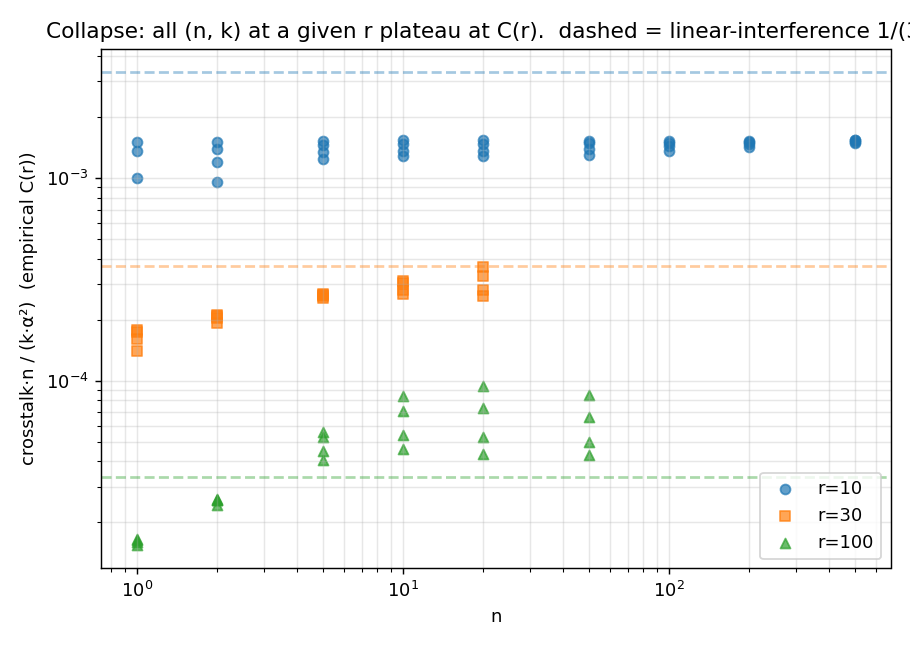
\includegraphics[width=0.80\textwidth]{figures/scaling_collapse_final.png}
\caption{Normalised cross-talk collapses at each ratio. Points are
all $(n, k)$ pairs for fixed-$p$-trained models; dashed lines are the
linear-interference prediction $1/(3r^2)$. Within each $r$, the residual
constant $C(r) = \text{crosstalk}\cdot n / (k\,\alpha^2)$ is flat across
$n$ (excluding $n{=}1$ outliers where $\Win$ is rank one).}
\label{fig:collapse}
\end{figure}

Collapsing $(\text{crosstalk}\cdot n)/(k\,\alpha^2)$ across the trained
models (Fig.~\ref{fig:collapse}) gives
\begin{equation}\label{eq:law}
\boxed{\;\text{crosstalk-per-output} \;\approx\; C(r)\cdot k\cdot\alpha^2/n\;}
\end{equation}
with ratio-only constant $C(r)$:

\begin{center}
\begin{tabular}{lcccc}
\toprule
$r$ & $C_{\text{obs}}$ & $1/(3r^2)$ & $\bar\rho\cdot 1/(3r^2)$ & $C_{\text{obs}}/[\bar\rho/(3r^2)]$ \\
\midrule
10  & $1.5\times 10^{-3}$ & $3.3\times 10^{-3}$ & $3.3\times 10^{-3}$ & $0.45$ \\
30  & $3.0\times 10^{-4}$ & $3.7\times 10^{-4}$ & ${\sim}4.5\times 10^{-4}$ & $0.67$ \\
100 & $5.0\times 10^{-5}$ & $3.3\times 10^{-5}$ & ${\sim}5.7\times 10^{-5}$ & $0.88$ \\
\bottomrule
\end{tabular}
\end{center}

\noindent The naive linear-interference prediction $1/(3r^2)$ underlies
Eq.~\eqref{eq:law}: sum of $k$ iid interferers, each with squared amplitude
$\alpha^2\Welch^2 \approx \alpha^2/(r^2 n)$, times $\mathrm{Var}(v)=1/3$.
The measured $C(r)$ is smaller than $\bar\rho/(3r^2)$ by a factor $\eta(r)$
that grows with $r$ ($0.45 \to 0.88$). I interpret $\eta(r)$ as ReLU
gating of interference, stronger at small $r$ where the hidden layer has
neurons to spare; this interpretation is inferred from the
decomposition, not independently verified.

\section{Fixed $p$: plateau}

\begin{figure}[h]
\centering
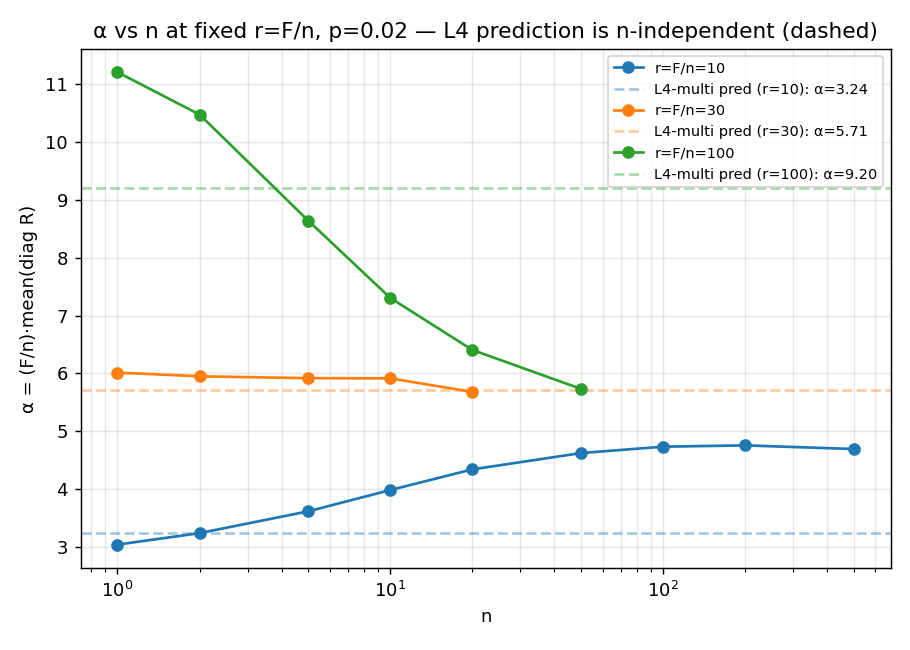
\includegraphics[width=0.49\textwidth]{figures/scaling_alpha_sat.png}
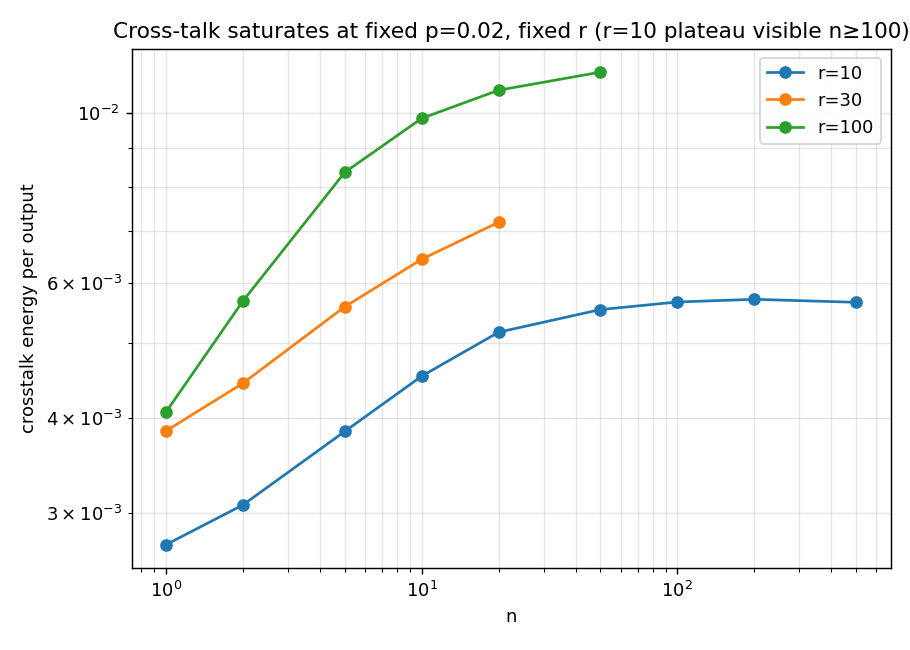
\includegraphics[width=0.49\textwidth]{figures/scaling_xtalk_fixed_p.png}
\caption{Left: $\alpha$ vs $n$ at fixed $r$, $p = 0.02$. Dashed lines
are the $L^4$ multi-feature prediction (Eq.~\ref{eq:L4}), which is
independent of $n$ at fixed $r, p$. Right: cross-talk per output vs $n$
at $p = 0.02$. At $r = 10$, both $\alpha$ and cross-talk flatten from
$n \ge 100$ (values at $n = 100, 200, 500$ agree to $\le 1\%$).}
\label{fig:fixed-p}
\end{figure}

At $r = 10$, $p = 0.02$:
\begin{center}
\begin{tabular}{l|rrrrrrrrr}
\toprule
$n$ & 1 & 2 & 5 & 10 & 20 & 50 & 100 & 200 & 500 \\
\midrule
$\alpha$ & 3.04 & 3.24 & 3.62 & 3.99 & 4.34 & 4.63 & 4.74 & 4.76 & 4.70 \\
$\text{crosstalk}{\times}10^3$ & 2.73 & 3.08 & 3.84 & 4.53 & 5.17 & 5.53 & 5.66 & 5.71 & 5.66 \\
\bottomrule
\end{tabular}
\end{center}

At $n{=}100,200,500$ the cross-talk values differ by $<1\%$ and $\alpha$
by $<2\%$. ``Saturation'' here means ``no growth observable over $5\times$
change in $n$''; with a single seed I cannot rule out a slow log drift.

At $r{=}100$, $p{=}0.02$, $\alpha$ drops from $11.2$ to $5.7$ over
$n{=}1..50$. Inspection of $R$ reveals $\rho$ growing from $1.0$ to
$2.0$: the optimiser cannot achieve a Welch-packed frame once
$pF > n$ (the overcrowded regime), and $R = \alpha P$ fails. This is
the main regime where the $\alpha$ prediction below breaks.

\section{Fixed $k$: $1/n$ decay}

\begin{figure}[h]
\centering
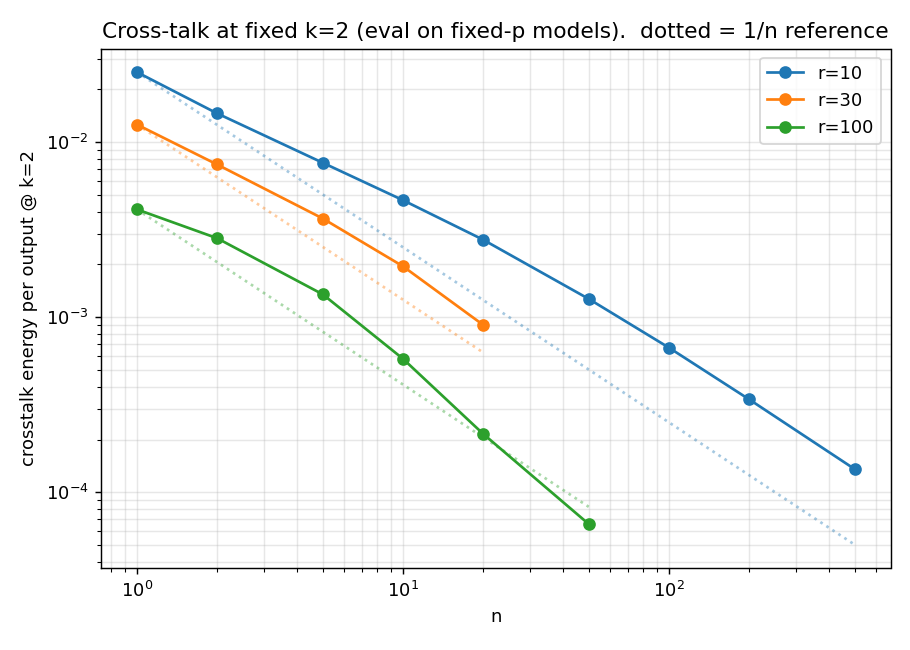
\includegraphics[width=0.65\textwidth]{figures/scaling_xtalk_fixed_k.png}
\caption{Cross-talk per output at fixed $k{=}2$ (evaluated on fixed-$p$
trained models). Dotted lines are $1/n$ references. The fit is clean
at all three ratios over three decades of $n$.}
\label{fig:fixed-k}
\end{figure}

At $r{=}10$, $k{=}1$, $(\text{crosstalk}\cdot n)/\alpha^2$ is constant
to $<5\%$ across $n{=}1..500$: $\{1.50, 1.51, 1.53, 1.54, 1.54, 1.52,
1.51, 1.50, 1.49\}\times 10^{-3}$.

This directly verifies the Elhage scaling: holding $k$ co-active
features fixed, per-output error decays as $1/n$ and vanishes with
width. For fixed $p = pF/F$ the count $k = pF$ grows linearly with $F$,
so Eq.~\eqref{eq:law} gives $C(r)\cdot p\cdot r\cdot \alpha^2$,
constant in $n$ (once $\alpha$ saturates).

\section{Closed-form prediction for $\alpha$}

Assume:
\begin{itemize}
  \item linear forward pass, $\hat y_i = \beta v_i + \sum_{j\in S\setminus i} R_{ij} v_j$,
  \item $R = \alpha P$ with $P$ rank-$n$ Parseval ($P_{jj} = n/F$),
  \item off-diagonals at Welch, $R_{ij}^2 \approx \alpha^2\Welch^2$,
  \item $\xi_i = \sum_j R_{ij} v_j$ approximately Gaussian, $\mathbb{E}[\xi^4] \approx 3\sigma^4$.
\end{itemize}
Computing $\mathbb{E}[(\hat y_i - \mathrm{ReLU}(x_i))^4]$ over
$v_j \sim \mathrm{Uniform}(-1,1)$ and summing over $i$, with
$u := \beta = \alpha n/F$, $r = F/n$, $\sigma^2 = p\alpha^2/(3r) = pu^2 r/3$:
\begin{equation}\label{eq:L4}
L^4(u; p, r) = \frac{p}{10} A(u) + \frac{p^2 r}{3} u^2 B(u) + \frac{p^2 r^2}{3} u^4
\end{equation}
with $A(u) = (u-1)^4 + u^4$, $B(u) = (u-1)^2 + u^2$. Minimise
numerically over $u \in (0, 1)$; the prediction depends on $(p, r)$ only
(\emph{not $n$}), and $\alpha^* = r\cdot u^*$.

\begin{figure}[h]
\centering
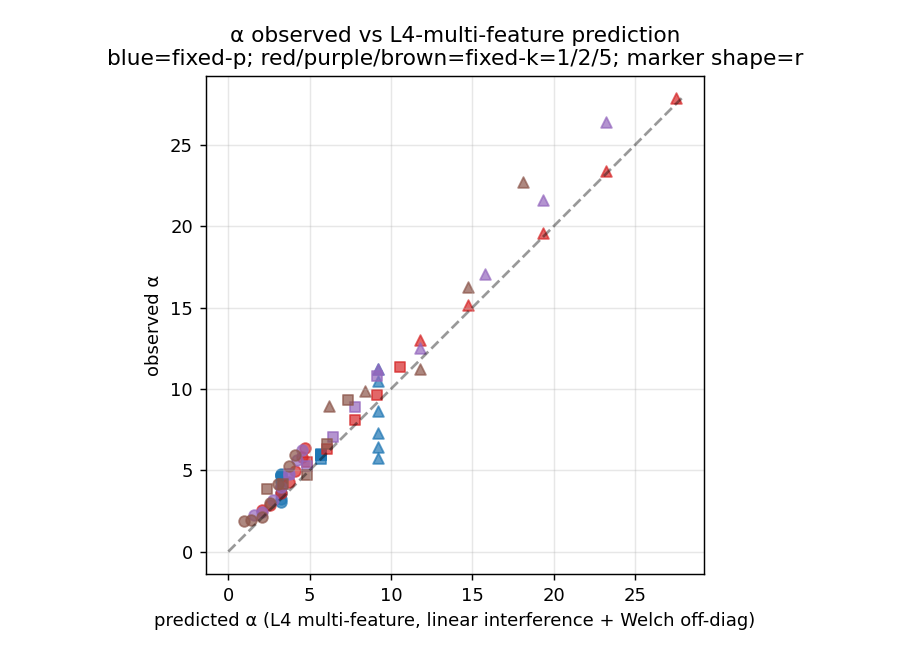
\includegraphics[width=0.60\textwidth]{figures/scaling_alpha_vs_pred.png}
\caption{Observed $\alpha$ vs Eq.~\eqref{eq:L4} prediction. Circle/square/
triangle marker = $r \in \{10, 30, 100\}$; colour = training regime
(blue $= $ fixed $p{=}0.02$; red/purple/brown $= $ fixed $k \in
\{1, 2, 5\}$). Dashed line $y{=}x$.}
\label{fig:alpha-pred}
\end{figure}

\noindent Accuracy (Fig.~\ref{fig:alpha-pred}):
\begin{itemize}
  \item Best apparent match at fixed-$k{=}1$, $r{=}100$, $n{=}10, 20$:
  predicted $23.26, 27.55$ vs observed $23.42, 27.88$ ($\le 1\%$). This
  match is partly coincidental: the Gaussian $\mathbb{E}[\xi^4]$ approx
  underweights the $\sigma^4$ penalty (the true value is
  $(3 + 9/(5k))\sigma^4$), while ReLU gating reduces effective $\sigma^2$
  below the Welch prediction. Both errors are non-trivial and point
  opposite.
  \item Fixed-$p$ at $r{=}30$: ratio $0.99$--$1.05$.
  \item Fixed-$p$ at $r{=}10$: ratio $1.0$--$1.5$ (observed $\alpha$
  higher, consistent with stronger ReLU gating).
  \item Fixed-$p$ at $r{=}100$ large $n$: ratio $0.62$--$0.79$ (the
  overcrowded regime $pF > n$ where $\rho > 1$).
\end{itemize}

\section{Summary and limits}

\paragraph{What was established.}
\begin{itemize}
  \item Cross-talk law Eq.~\eqref{eq:law} with $C(r)$ extractable from
  data across $\sim 70$ models.
  \item $1/n$ decay at fixed $k$, fixed $r$: verified $\le 5\%$ over
  $n=1..500$ at $r{=}10$.
  \item Plateau at fixed $p$, fixed $r$: verified flat to $\le 1\%$
  at $r{=}10$, $n = 100..500$.
  \item Closed-form $\alpha^*(p, r)$ from $L^4$ multi-feature
  derivation, matching $\le 5\%$ in the Welch-saturated (small-$p$)
  regime.
\end{itemize}

\paragraph{What was not established / open.}
\begin{itemize}
  \item Seed robustness: single seed per config. No error bars.
  \item $\eta(r)$ interpretation: inferred from $C(r)/[\bar\rho/(3r^2)]$,
  not independently measured.
  \item Gaussian $\xi^4$ assumption is asymptotic in $k$; at $k{=}1$ the
  correction is $60\%$ and the fixk1 match benefits from cancellation.
  \item $r{=}100$ $n$-dependence of $\alpha$: ansatz breaks when $pF > n$.
  \item Stacked-layer error: single layer only. Whether the measured
  per-layer noise is small enough for a realistic downstream corrector
  is not addressed here.
\end{itemize}

\paragraph{Error-correction implication.} Two regimes sit on opposite sides
of a clean boundary:
\begin{itemize}
  \item Fixed fraction of co-active features: per-layer cross-talk
  plateaus; width alone does not help.
  \item Fixed count of co-active features: per-layer cross-talk decays
  as $1/n$; width does help.
\end{itemize}
Whether a stacked superposition network lives in one or the other is a
modelling choice about the downstream distribution.

\paragraph{Artifacts.}
Source: \texttt{scaling/\{measure\_mse.py, train\_ratios.py,
train\_fixed\_k.py, train\_r10\_large.py, measure\_fixk.py, check\_R.py,
alpha\_theory.py, final\_plots.py\}}. Data:
\texttt{data/scaling\_mse*.json}, \texttt{data/R\_structure.json}.
Figures: \texttt{figures/scaling\_\{alpha\_sat, xtalk\_fixed\_p,
xtalk\_fixed\_k, collapse\_final, alpha\_vs\_pred\}.png}. Concise
Markdown report: \texttt{SCALING\_REPORT.md}.

\end{document}
